\documentclass[12pt]{article}

\usepackage{fullpage}
\usepackage{datetime}
\usepackage{amsfonts}

\usepackage{graphicx}
\usepackage{subcaption}

\usepackage{biblatex}
\addbibresource{./references.bib}

\title{
  Learning Neural Orientation Field for Volumetric Hair Reconstruction \\
  {
    \small
    Project Milestone
  }
}
\author{
  Fangjun Zhou \\ fzhou48
  \and Weiran Xu \\ weiran
  \and Zhenyu Zhang \\ zhenyuz5
}
\date{\today}

\begin{document}
  \maketitle

  \section{Introduction}
  % Project motivation

  Reconstructing human hair is one of the most challenging yet critical process in rendering photorealistic digital human. Unlike other parts of the human body, human hair is highly detailed and often intertwined together. Therefore, it's difficult to use traditional photogrammetry method to reconstruct its structure.

  Before machine learning model is used in this field, artists often hand crafted splines on skulls to represent hair strands. Each strand is then textured and rendered to mimic the hair volume. This workflow requires a lot of experience as it's non-trivial for artists to infer the final render result from hair stand splines. To reduce the workload and improve the accuracy of hair reconstruction, machine learning models are trained to generate hair strand from captured images.

    In this work, we propose a new method capturing the hair structure by a 3D vector field from $\mathbb{R}^{3} \rightarrow \mathbb{R}^{3}$ representing the hair growing direction and occupancy. This mapping can be used later to generate hair stand directly by numerically solving the PDE. It can also be used as a latent variable to guide other generative models as mentioned in \cite{metzer_latent-nerf_2022}. We can fit this vector field by a simple MLP. We then project the vector field onto multiple camera view with a volumetric renderer. Since the screen space projection and volumetric rendering algorithm are differentiable, we are able to learn the vector field from images from multiple camera angle.

  \section{Related Work}

  Previous attempt to achieve this goal mainly focus on learning based hair strand generation. This includes some studies about single view hair synthesis \cite{saito_3d_2018, zheng_hairstep_2023, wu_neuralhdhair_2022, ma_single-view_nodate}. Since the image only contains hair structure from one viewing angle, it's impossible to reconstruct entire hair accurately. These models often use pretrained image encoders such as ResNet-50 \cite{saito_3d_2018} to encode the abstract hair style into a feature vector, then use generative models such as U-Net \cite{zheng_hairstep_2023}, VAE \cite{saito_3d_2018}, and diffusion models \cite{sklyarova_neural_2023} to generate the final strand. These models also struggle with generating curly hair as there's only limited information about growing direction after feature extraction.

  In \cite{sklyarova_neural_2023} and \cite{rosu_neural_2022}, the authors also tried hair syntheses from multi-view images. However, these two studies still failed to capture finer detail.

  Another study about this topic tried to tackle this problem by expanding the traditional PatchMatch MVS (PMVS) algorithm to a Line-based PatchMatch MVS (LPMVS) \cite{nam_strand-accurate_nodate}. This method, despite its high accuracy, doesn't capture the volumetric property of human hair.

  Our work is highly inspired by NeRF \cite{mildenhall_nerf_2020}, a model used for 3D reconstruction from 2D images. However, our model differs in two major way.

  In NeRF, the model fits a radiance field from $\mathbb{R}^{5} \rightarrow \mathbb{R}^{4}$. The input of the randiance function includes the sample position and view direction. However, since the vector field our model fits is view-independent, the input space is only $\mathbb{R}^{5}$. This makes it easier for the model to capture more information from a smaller dataset.

  On top of that, the volumetric renderer on vector field also differs from the one on radiance field. In this case, NeRF only integrate the sampled radiance for each ray, while our model need to project the sample vector onto the filming plane an then integrate the projected vector.

  \section{Method}
    \subsection{Data Preprocess}
    
    Our model will be trained on a set of images of human bust from multiple viewing angles.

    $\mathbf{Image:}$  For each of the images, the preprocessing kernel will extract the projection of the hair growing direction onto the camera viewing plane. In this paper, we utilize the preprocessing pipeline in HairStep \cite{zheng_hairstep_2023} to segment out the hair from the image and get the direction vector field of the top layer hair. Each pixel in the preprocessed image has three channels rgb, we use r channel = 255 to denote the pixel belongs to the hair region, and the g and b channel together as the direction vector. For the region that does not belongs to hair but belongs to human body, its rgb = (127, 0, 0), and for other region we set rgb to $\mathbf{0}$.
    \begin{figure}[h]
        \centering
        % first col
        \begin{subfigure}{0.2\textwidth}
            \centering
            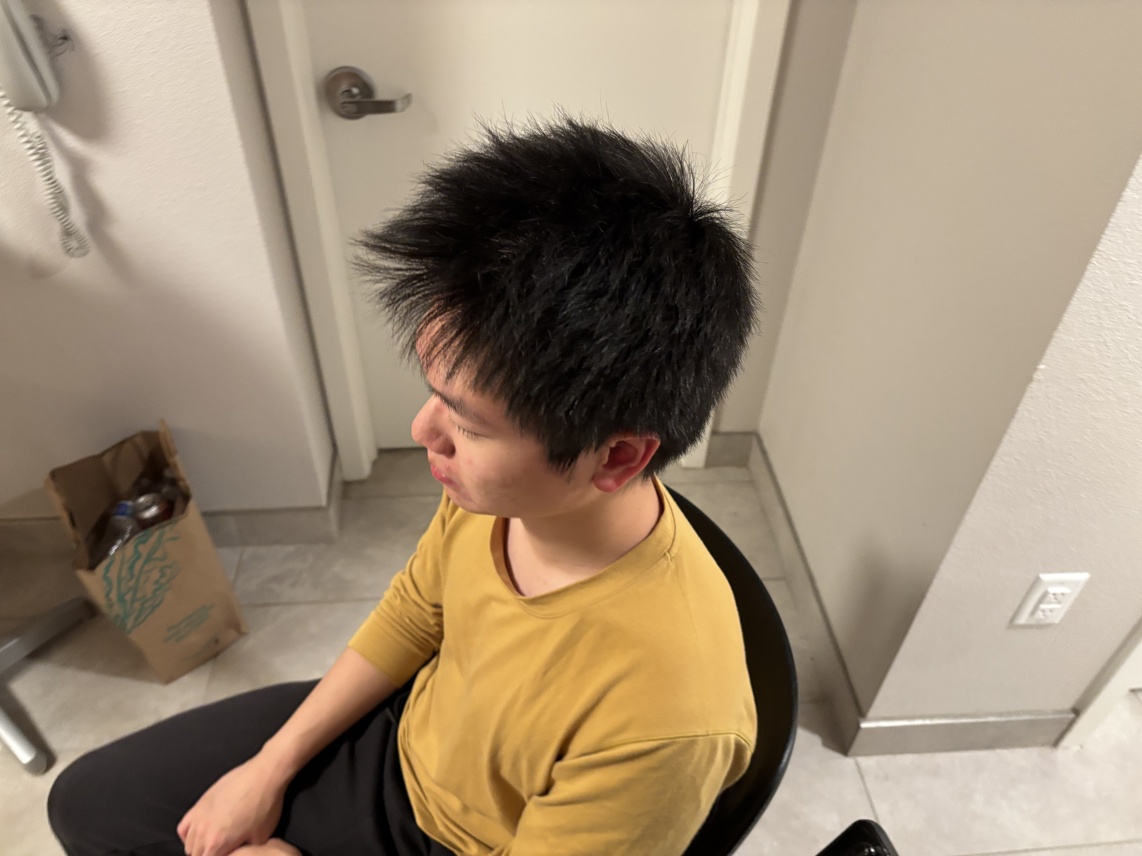
\includegraphics[width=\textwidth]{project-milestone/images/portrait_raw/IMG_0342.png}
            \caption{raw}
        \end{subfigure}
        \hfill
        \begin{subfigure}{0.2\textwidth}
            \centering
            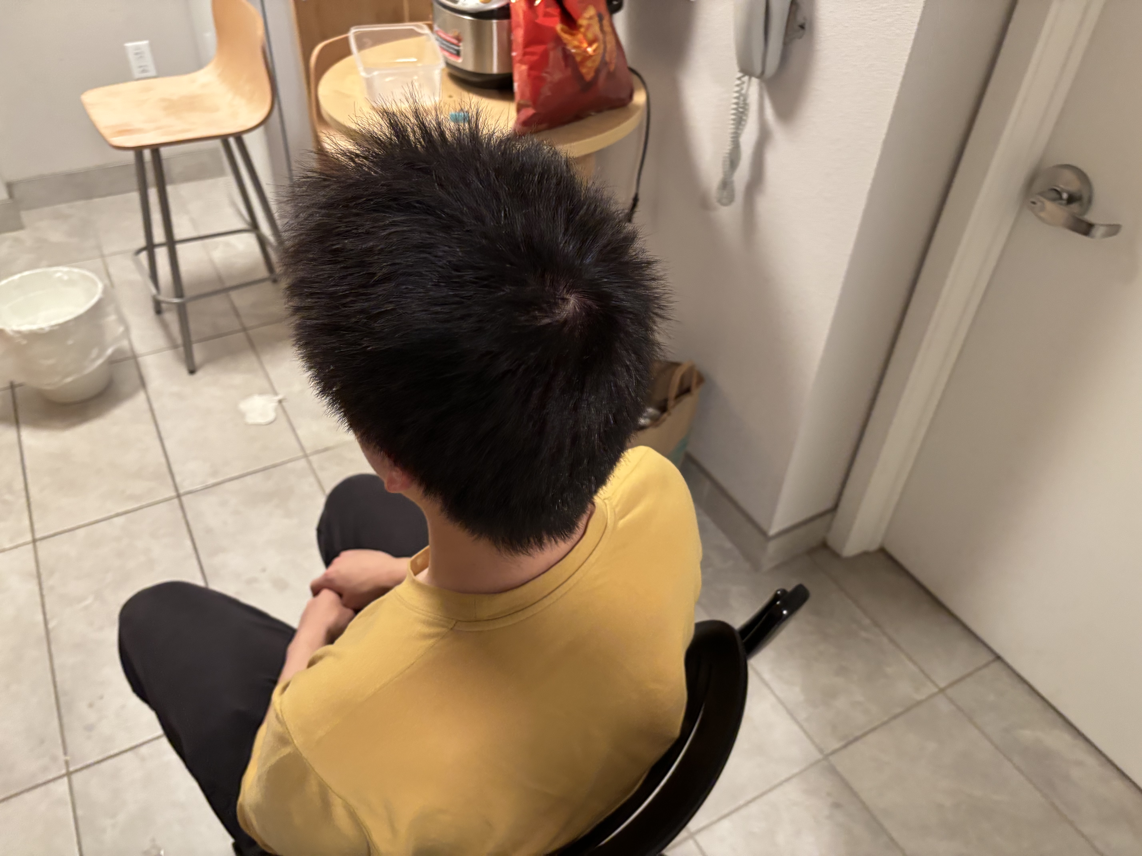
\includegraphics[width=\textwidth]{project-milestone/images/portrait_raw/IMG_0346.png}
            \caption{raw}
        \end{subfigure}
        \hfill
        \begin{subfigure}{0.2\textwidth}
            \centering
            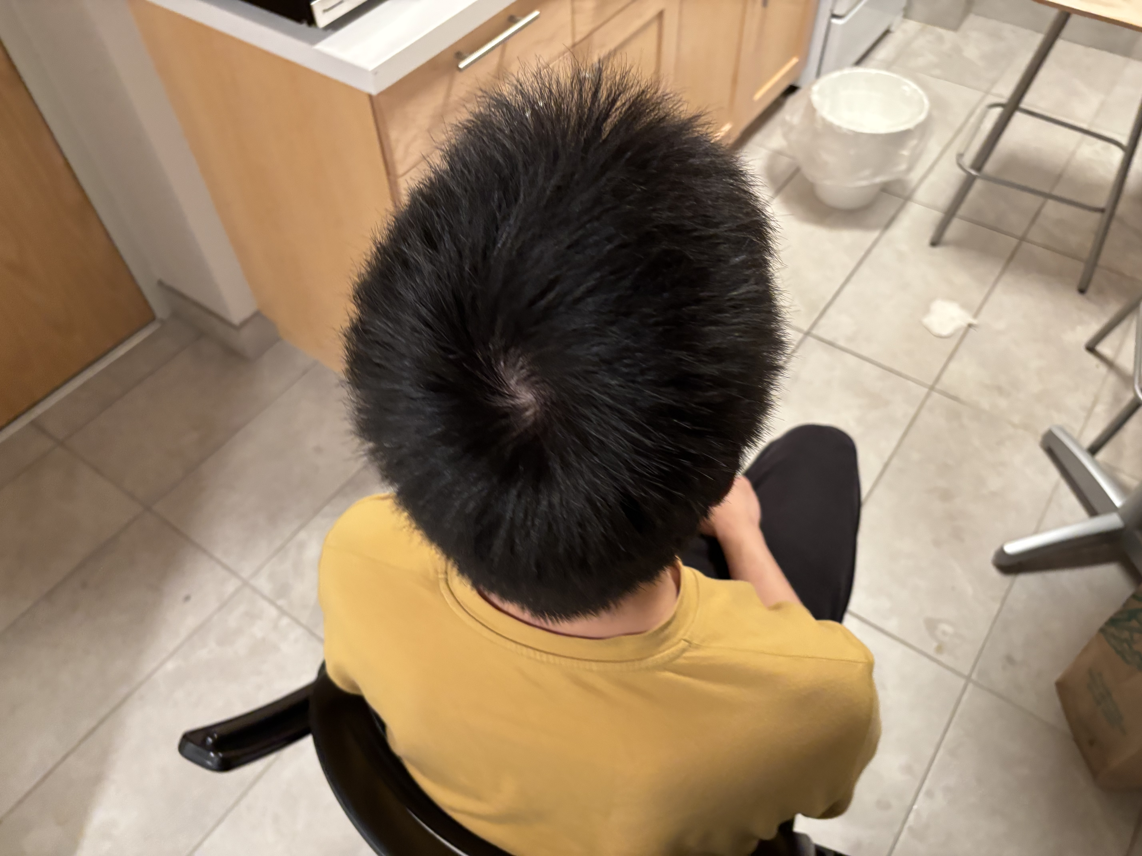
\includegraphics[width=\textwidth]{project-milestone/images/portrait_raw/IMG_0349.png}
            \caption{raw}
        \end{subfigure}
        \vskip\baselineskip
        % second col
        \begin{subfigure}{0.2\textwidth}
            \centering
            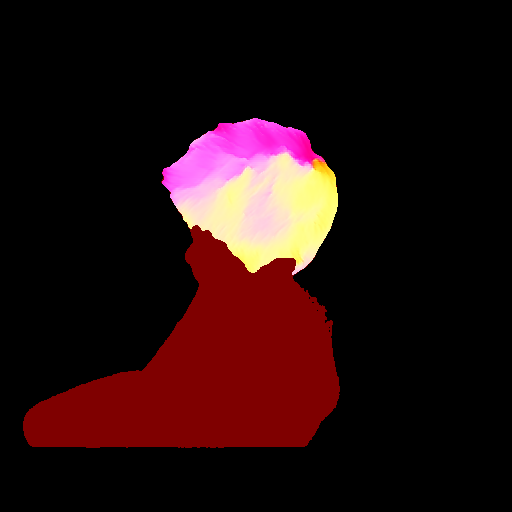
\includegraphics[width=\textwidth]{project-milestone/images/strand_map/IMG_0342.png}
            \caption{processed}
        \end{subfigure}
        \hfill
        \begin{subfigure}{0.2\textwidth}
            \centering
            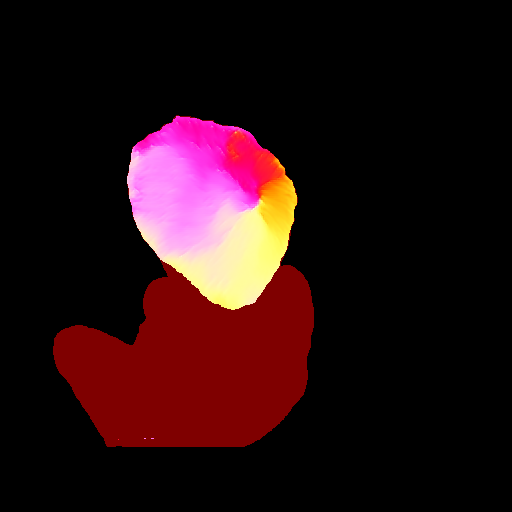
\includegraphics[width=\textwidth]{project-milestone/images/strand_map/IMG_0346.png}
            \caption{processed}
        \end{subfigure}
        \hfill
        \begin{subfigure}{0.2\textwidth}
            \centering
            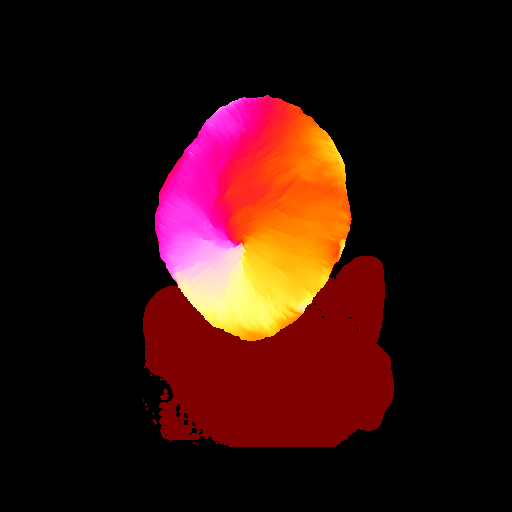
\includegraphics[width=\textwidth]{project-milestone/images/strand_map/IMG_0349.png}
            \caption{processed}
        \end{subfigure}
        
        \caption{Image Preprocessing}
        \label{fig:image_prep}
    \end{figure}

    $\mathbf{Camera:}$ For portrait taken in reality, we use COLMAP, a general-purpose MVS pipeline that processes a set of images to generate a point cloud, to reconstruct the camera position and angle. We also implemented a visualizer for COLMAP. In Figure \ref{fig:colmap_demo}, we see that COLMAP successfully reconstruct camera for the image.
    \begin{figure}[h]
        \centering
        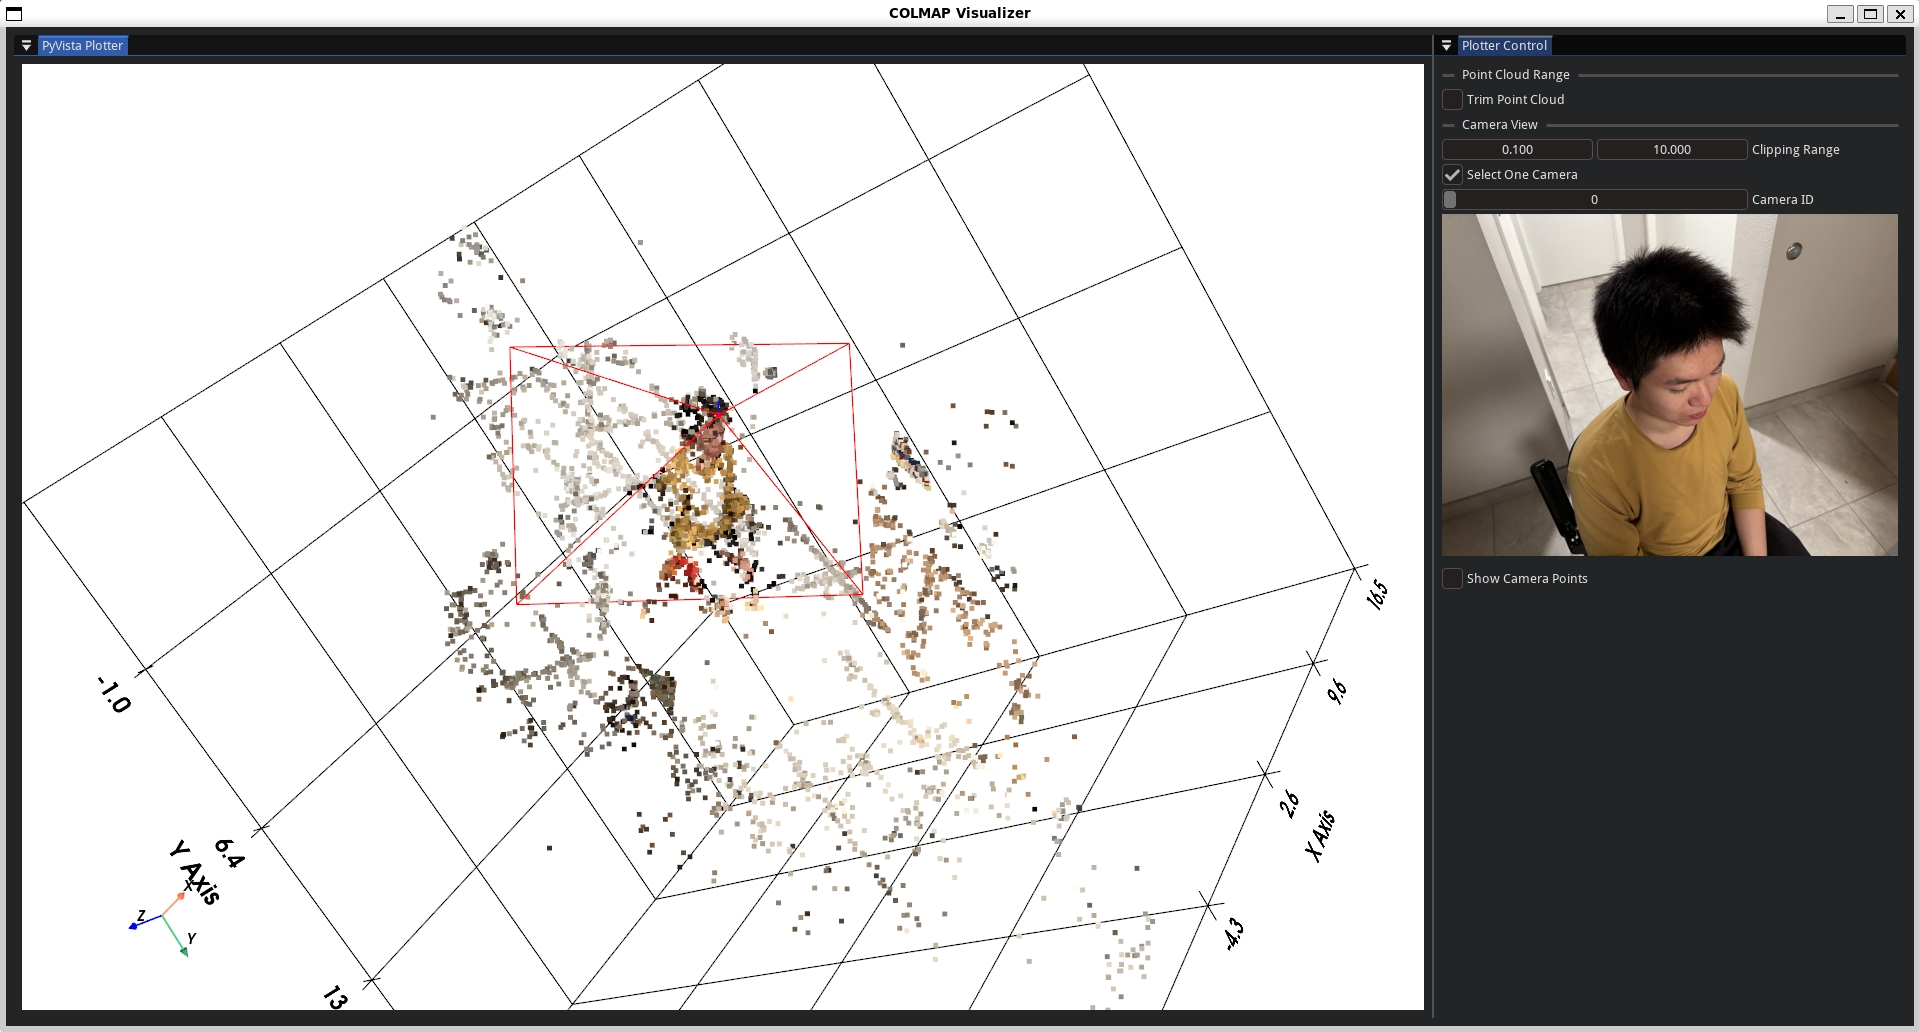
\includegraphics[width=0.5\linewidth]{project-milestone/images/colmap_demo.png}
        \caption{Camera position reconstruction using COLMAP}
        \label{fig:colmap_demo}
    \end{figure}

    \subsection{Training}

    Add nerf tuning here.
    
    \subsection{Backbone}
    
    The backbone network is similar to NeRF \cite{mildenhall_nerf_2020}'s backbone, primarily consisting of multiple MLP layers and residual connections. The difference is that the input to the network we constructed is the spatial coordinates $(x, y, z)$ of the point to be evaluated, and the output is the direction vector of the hair at that point $v = (v_x, v_y, v_z)$, as well as the opacity parameter $\sigma$. The direction vector is used to describe the growing direction of the hair at this point, while the opacity parameter sigma is used in loss construction to model the occlusion relationships of the hair which will be discussed later.
    
    \subsection{Loss Definition}
    
    The construction of the model's loss is divided into two parts: occlusion relationship modeling and plane projection of the direction vector. In occlusion relationship modeling, the weighted 3D direction vector is obtained by integrating the direction vectors along the observation direction ray, weighted by the opacity parameter $\sigma$ and an function describe the accumulative transmittance, similar to NeRF \cite{mildenhall_nerf_2020}. We can simulate the integration process through sampling specific points on the observation direction ray and discrete the original integral.

    For the second part, we project the weighted 3D direction vector obtained from the first part along the viewing direction onto the camera plane, resulting in the 2D direction vector observed by the camera. The final loss function is constructed by calculating the MSE loss between the 2D direction vector and the ground truth. We will use mini-batched gradient descent to optimize the loss function.
    
  \section{Experiment}

  Given a set of images of human busts from multiple viewing angles, we first use COLMAP as our baseline. Next, we will evaluate the quality enhancements provided by our model compared to both the Line-based PatchMatch MVS \cite{nam_strand-accurate_nodate} and generative models. Since the final output of our model differs from that of \cite{nam_strand-accurate_nodate} and the generative models, we will not compare their performances directly. Instead, we will evaluate performance relative to COLMAP. Finally, we will demonstrate the tunability of our model's output using Blender.

  $\mathbf{Metrics:}$ Peak Signal-to-Noise Ratio (PSNR) is a metric from signal processing to evaluate similarity between images, often used in image reconstrction. PSNR is essentially a 2D MSE. Learned Perceptual Image Patch Similarity (LPIPS) is a metric measure how human may perceive the similarity of different images, it is robust to noise and focus on higher level features.
  
  % Intended experiment
  

  \printbibliography

\end{document}
